%\phantomsection
\sectionmark{Buca bidimensionale}
\section{Buca di potenziale bidimensionale a pareti infinite}
\sectionmark{Buca bidimensionale}

Il calcolo delle funzioni d'onda è, in questo caso, abbastanza 
semplice da non richiedere l'aiuto di metodi numerici
o di strumenti informatici\footnote{
  Ciò non toglie che, anche nell'affrontare questo problema,
  \emph{Maxima}\cite{MAXIMA} sia stato un utile strumento di verifica,
  ad esempio per controllare le condizioni di normalizzazione.
}, dei quali ci serviremo solo per la 
rappresentazione grafica.

%{\scriptsize
%Per illustrare questa tecnica con un primo esempio, si considerino i 
%seguenti grafici della funzione $\zeta(x+iy)$ nei 
%domin\^i $[0,3]\times[-5,50]$ e
%$\left[-\frac{7}{2}, \frac{7}{2}\right] \times \left[-40, 40\right]$
%(quest'ultimo in scala logaritmica), ove $\zeta$ è la 
%\emph{funzione-zeta di Riemann} definita come 
%$\zeta(s) = \sum_{n=1}^\infty \frac{1}{n^s}$, con $s\in\mathbb{C}$.
%}
%
%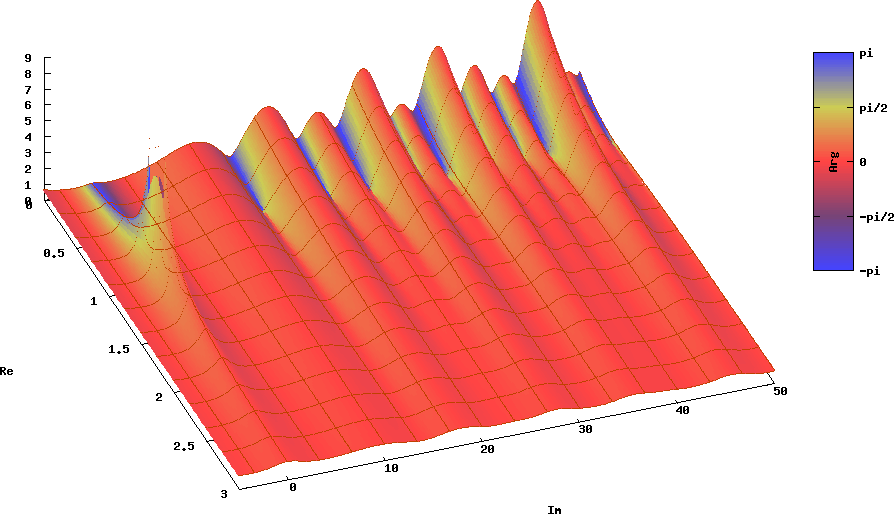
\includegraphics[width=60mm,height=30mm]{img/z/z0.png}
%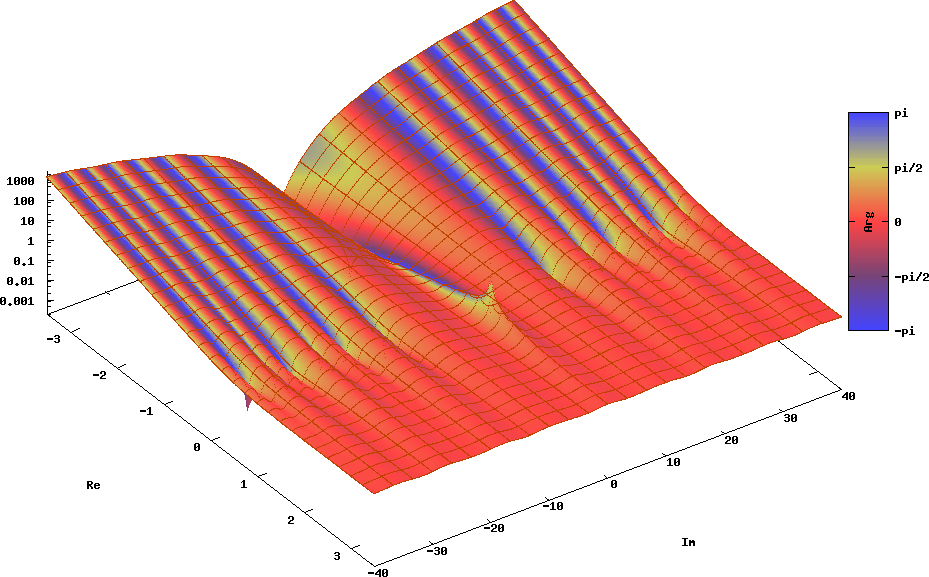
\includegraphics[width=60mm,height=36mm]{img/z/zwhole5.png}
 


\subsection{Combinazioni lineari finite}

Sceglieremo ora alcune combinazioni lineari, opportunamente normalizzate,
delle funzioni \eqref{eq:evol_autofunzioni}:
\begin{subequations}\label{eq:combinaz}\begin{gather}
    \sqrt{\frac{1}{ 5}}\Psi_{11}  + 
    \sqrt{\frac{2}{ 5}}\Psi_{21}  + 
    \sqrt{\frac{2}{ 5}}\Psi_{12}  , \label{eq:comb1} 
  \\
    \sqrt{\frac{1}{ 5}}\Psi_{11}  + 
    \sqrt{\frac{2}{ 5}}\Psi_{21}  + 
  i \sqrt{\frac{2}{ 5}}\Psi_{12}  , \label{eq:comb2} 
  \\
    \sqrt{\frac{1}{10}}\Psi_{11}  + 
    \sqrt{\frac{3}{10}}\Psi_{21}  + 
  i \sqrt{\frac{3}{10}}\Psi_{12}  +
    \sqrt{\frac{3}{20}}\Psi_{32}  + 
  i \sqrt{\frac{3}{20}}\Psi_{23}  , \label{eq:comb3}  
  \\
    \sqrt{\frac{3}{10}}\Psi_{11}  + 
    \sqrt{\frac{3}{10}}\Psi_{22}  + 
    \sqrt{\frac{1}{ 5}}\Psi_{52}  +
  i \sqrt{\frac{1}{ 5}}\Psi_{25}  . \label{eq:comb4}
\end{gather}\end{subequations} 
%
Ci occorrerà salvare in un file ciascuna
di queste definizioni. Ad esempio, l'ultima delle \eqref{eq:combinaz}, 
tenuto conto della \eqref{eq:evol_autofunzioni} e della \eqref{eq:phi}, 
nella sintassi di \emph{Gnuplot}\cite{GNUPLOT} diventa:
\begin{lstlisting}

set zrange[0:.80]

psi(x,y)=(2./pi)*(\
    cos(1*x)*cos(1*y)*exp(- 2*i*t)         *sqrt(.30)+\
    sin(2*x)*sin(2*y)*exp(- 8*i*t)         *sqrt(.30)+\
    cos(5*x)*sin(2*y)*exp(-29*i*t)         *sqrt(.20)+\
    sin(2*x)*cos(5*y)*exp(-29*i*t) *i      *sqrt(.20)\
)

\end{lstlisting}

\subsection{Simulazioni}

Lo script in \S\ref{sec:buca2d.anima.pl} accetta come argomento
il nome o il percorso di un file del tipo appena descritto
e riportato in \S\ref{sec:myfunc.gpi}. Questo file
contiene la definizione della funzione d'onda e l'impostazione
del \emph{range} di valori per la rappresentazione grafica. 

Lo script crea una directory nella quale salverà le immagini prodotte;
carica un ``preambolo'' di impostazioni per \emph{Gnuplot} (si veda 
\S\ref{sec:buca2d.preamble.gpi}); dopo di che itera il disegno
dei grafici su un insieme discreto di valori del tempo $t$.
\begin{lstlisting}

for($t=$t_i;$t<=$t_f;$t+=$step) {
    $n=sprintf("%07.4f",$t);
    $progress=sprintf("%02d", (($t-$t_i)/($t_f-$t_i))*100 );
    print STDERR "plotting @ t=$n  $progress\%     \r";
    print GNUPLOT "
        set title \"t=$n\" offset 0,-1
        t=$t
        set output \"$dir/frame.$n.$format\"
        load \"$plot\"
    ";
}

\end{lstlisting}
Nel precedente frammento di codice, \texttt{\$plot} è
il nome di un ulteriore file (v. \S\ref{sec:buca2d.plot.gpi}) contenente le 
istruzioni con cui \emph{Gnuplot} effettua il disegno vero e proprio.
\begin{lstlisting}

# pseudodata special file '++'
# requires Gnuplot 4.3 or higher (currently under development, 
# available via CVS only -- @ 2008-06-25)
#
# http://gnuplot.sourceforge.net/demo_4.3/heatmaps.3.png
#
# http://sourceforge.net/tracker/index.php?func=detail&
# aid=1872528&group_id=2055&atid=302055
#

splot '++' using 1:2:(abs(psi($1,$2))**2):(arg(psi($1,$2))) w pm3d at s

\end{lstlisting}
L'ultima istruzione, grazie ad una recente caratteristica, consente 
l'uso diretto del colore per rappresentare l'argomento complesso 
della funzione d'onda.\footnote{ Nelle precedenti versioni 
di \emph{Gnuplot} sarebbe stato necessario creare un \emph{file di dati}
con un programma esterno.}

Con le impostazioni scelte, al termine dell'esecuzione 
troviamo nella directory creata oltre 1500 immagini,
sufficienti a produrre un'animazione \footnote{
  Per convertire una sequenza di immagini in un file video si possono
  usare strumenti quali \emph{MEncoder}/\emph{MPlayer}  
  \url{http://www.mplayerhq.hu/}.
}
della durata di circa un minuto allo standard 
di 25 frame$/s$.

\subsection{Immagini ed esemp\^{i}}

Il comportamento della \eqref{eq:comb1} in \figurename~\ref{fig:comb1} 
ricorda quello di una particella
che ``va avanti e indietro'' lungo la diagonale del quadrato
$[-\frac{\pi}{2}, \frac{\pi}{2}]^{2}$.
\begin{figure}\begin{center}
  \subfloat[]{
  \includegraphicshp{img/buca2d/1/1.png} 
  } \\ 
  \subfloat[]{
  \includegraphicshp{img/buca2d/1/2.png}
  }
  \caption{Buca 2D: $                 %
      \sqrt{\tfrac{1}{ 5}}\Psi_{11}  + %
      \sqrt{\tfrac{2}{ 5}}\Psi_{21}  + %
      \sqrt{\tfrac{2}{ 5}}\Psi_{12}    %
  $.}
  \label{fig:comb1}
\end{center}\end{figure}

La \eqref{eq:comb2}, rappresentata in \figurename~\ref{fig:comb2},
è diversa dalla \eqref{eq:comb1} solo per
un fattore $i$ (unità immaginaria) nel coefficiente relativo
a $\Psi_{12}$, ma il comportamento è molto diverso: la particella
sembra ``ruotare'' attorno al centro della buca.
\begin{figure}\begin{center}
  \subfloat[]{
    \includegraphicshp{img/buca2d/2/1.png}
  } \\
  \subfloat[]{
    \includegraphicshp{img/buca2d/2/2.png}
  } 
  \caption{Buca 2D: $                 %
      \sqrt{\tfrac{1}{ 5}}\Psi_{11}  + %
      \sqrt{\tfrac{2}{ 5}}\Psi_{21}  + %
    i \sqrt{\tfrac{2}{ 5}}\Psi_{12}    %
  $.}
  \label{fig:comb2}
\end{center}\end{figure}

La \eqref{eq:comb3} in \figurename~\ref{fig:comb3} 
mostra un comportamento misto.
\begin{figure}[p]\begin{center}
  \includegraphicshp{img/buca2d/3/1.png}
  \caption{Buca 2D: $                 %
      \sqrt{\tfrac{1}{10}}\Psi_{11}  + %
      \sqrt{\tfrac{3}{10}}\Psi_{21}  + %
    i \sqrt{\tfrac{3}{10}}\Psi_{12}  + %
      \sqrt{\tfrac{3}{20}}\Psi_{32}  + %
    i \sqrt{\tfrac{3}{20}}\Psi_{23}    %
  $.}
  \label{fig:comb3}
\end{center}\end{figure}

La \eqref{eq:comb4}, rappresentata in \figurename~\ref{fig:comb4},
esibisce invece proprietà squisitamente ondulatorie.
\begin{figure}[p]\begin{center}
  \includegraphicshp{img/buca2d/4/1.png}
  \caption{Buca 2D: $                 %
      \sqrt{\tfrac{3}{10}}\Psi_{11}  + %
      \sqrt{\tfrac{3}{10}}\Psi_{22}  + %
      \sqrt{\tfrac{1}{ 5}}\Psi_{52}  + %
    i \sqrt{\tfrac{1}{ 5}}\Psi_{25}    %
  $.}
  \label{fig:comb4}
\end{center}\end{figure}

Anche per queste simulazioni, tutto il materiale multimediale,
il codice sorgente ed eventuale documentazione aggiuntiva
sono disponibili su \cite{PQ-QP}, alla pagina delle
\emph{Simulazioni}.

\subsection{Possibili sviluppi} \label{subsec:buca2d_sviluppi}

Combinando un piccolo numero di autofunzioni è difficile
ottenere qualcosa che ricordi un comportamento classico.
Poiché il raffronto fra il comportamento ondulatorio e quello
corpuscolare può essere molto istruttivo, potremmo
immaginare di invertire l'approccio al problema: considerare
cioè un pacchetto d'onda ben localizzato in un arbitrario
punto della buca con le opportune proprietà, e in seguito
calcolarne i coefficienti di Fourier rispetto alla 
base \eqref{eq:autofunz_buca}, magari con l'ausilio
di un programma per il calcolo. A questo punto si potrà
simularne l'evoluzione temporale in modo analogo 
(a meno di accorgimenti tecnici) a quanto fatto per le 
\eqref{eq:combinaz}.

